% Report
\documentclass{article}

% Here set the various packages
% Packages to load
\usepackage[english]{babel}
% %%% Support some german text
% \usepackage{ngerman}
% \usepackage[latin1]{inputenc}   % für Umlaute
%%%
% \usepackage[utf8]{inputenc}
\usepackage[T1]{fontenc}
\usepackage{microtype}

%%%
% \usepackage[inline]{enumitem} % Required for the "description" list.

%%% Fix for not hyperlinking citations
\makeatletter
\let\NAT@parse\undefined
\makeatother
\usepackage{hyperref}
% 
\usepackage{cite}
% \ifx\pdfoutput\undefined
% 	\usepackage{graphicx}
% \else
% 	\usepackage[pdftex]{graphicx}
% \fi
\usepackage{graphicx}
\graphicspath{{Figures/}}
\usepackage{amsmath}
% \interdisplaylinepenalty=2500

% Shading of questions. Use the "shaded" environment or the "\hl{}" command.
\usepackage{framed}
% \usepackage[dvipsnames]{color}
\usepackage[svgnames]{xcolor}
\usepackage{soul}
% Nice colours: Gainsboro, LightGoldenrod, LightSteelBlue
% furter ref: https://www.latextemplates.com/svgnames-colors
\definecolor{shadecolor}{named}{Gainsboro}
\sethlcolor{Gainsboro}

%%% Todo margin notes (enable/disable)
\usepackage{todonotes}
% \usepackage[disable]{todonotes}
%%%

%eof

%%%

\title{Programming of Supercomputers\\Worksheet 2}
\author{Oleksandr Voloshyn\\ Qunsheng Huang\\ Tommaso Bianucci}
\date{\today}

\begin{document}

\maketitle
\renewcommand{\abstractname}{Group members's contributions}
\begin{abstract}
	% Here write the contributions of the members of the group
	Here briefly state the contributions of the different members of the group!
\end{abstract}

\section{Task 1}
\subsection{Concepts description}
\begin{description}
	\item[Race condition] www
	\item[Deadlock] www
	\item[Heisenbug] www
	\item[Cache coherency and false sharing] www
	\item[Load imbalance] www
	\item[Amdahl's law] www
	\item[Parallelization overhead] www
	\item[Floating-point arithmetic challenges]
		\begin{enumerate}[label=\Alph*]
			\item Comparisons
		\end{enumerate}
\end{description}
Lorem ipsum

% Figure example
\begin{figure}[h!] % h=here, t=top, b=bottom, p=(extra)page, !=force
 	\begin{center}
 		
\includegraphics[width=.9\linewidth]{figure.png} % It searches in the Figures/ folder!
 		\caption{Caption text}
 		\label{fig:figureLabelName}
 	\end{center}
\end{figure}

\section{Task 2}

\subsection{Include a brief description of the following aspects of TotalView’s GUI in the report:}
\begin{itemize}
	\item Session Manager
	Manages debuggin sessions, see Fig.\ref{fig:sess_manager}. Displays previously configured debugging systems---allowing editing, copying and deleting of preivous settings, and view their respective configuration setups. Availble configurations include type of session (parallel/sequential), parallel implementation (poe-linux/MPICH etc.), number of parallel processes, number of nodes, environmental variables and input to parallel program upon startup.
	\begin{figure}[p] % h=here, t=top, b=bottom, p=(extra)page, !=force
			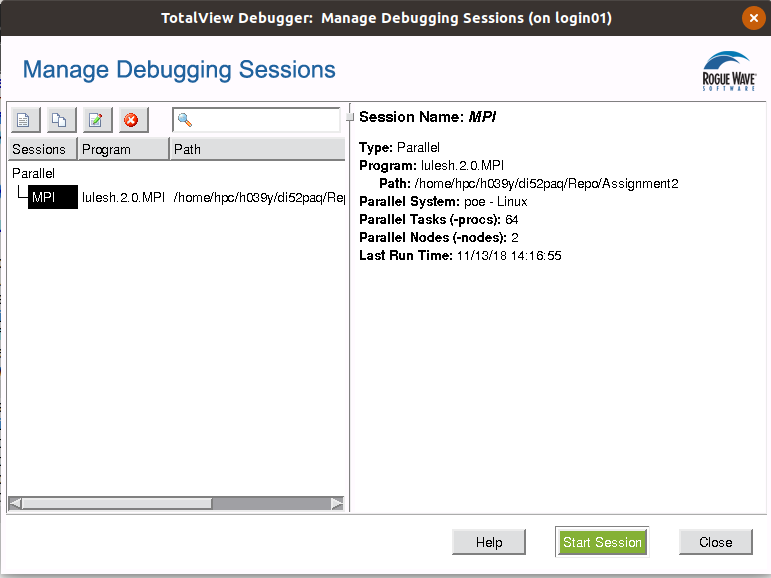
\includegraphics[width=.7\linewidth]{SessionManager.png}
		\caption{Session Manager}
		\label{fig:sess_manager}
	\end{figure}
	\item Root Window
	Lists all processes and threads controlled by TotalView, see \ref{fig:root_window}. Allows user to "Dive" into processes easily, which launches a process window for the selected process. Allows grouping of threads/processes for easier debugging.
		\begin{figure}[p] % h=here, t=top, b=bottom, p=(extra)page, !=force
			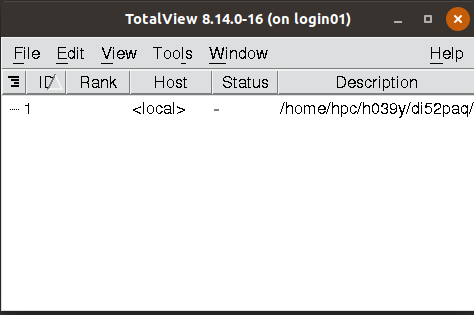
\includegraphics[width=.7\linewidth]{RootWindow.png}
		\caption{Root Window}
		\label{fig:root_window}
	\end{figure}
	\item Process Window
	Window for one specific process or thread, see Fig. \ref{fig:proc_window}. Provides information on state of the process and its individual threads. Information provided lsited in the various panes below.
	\begin{itemize}
		\item Stack Trace Pane
		Displays the call stack with any active threads, ie lists the active subroutines of the active thread. Able to move up and down the call stack by clicking on the stack frame (routine name) of interest. Stack Frame pane and Source pane updated for the specific routine when it is selected.
		\item Stack Frame Pane
		Displays information on the current thread's variables, ie allows users to see the current/stored values in existing variables.
		\item Source Pane
		Displays the source code for the main() function of the thread, process or selected routine
		\item Action Points, Processes, Threads Pane
		\begin{itemize}
		\item Process Tab: The processes tab, or Ranks tab for MPI programs, contains a grid. Each block in the grid represents one process. The color of the respective segments indicates the state of the process. 
		\item Threads Tab: The Threads Tab displays information about the state of your threads. Clicking on a thread tells TotalView to shift the focus within the Process Window to that thread.
		\item Actions Points Tab: Action points are specific actions performed when a particular source line is reached. There are four possible actions: breakpoints, barrier points, eval points, and watch points. Totalview assigns unique ID numbers for each action point, these are seen in the actions points tab
		\end{itemize}
	\end{itemize}
	\begin{figure}[p] % h=here, t=top, b=bottom, p=(extra)page, !=force
			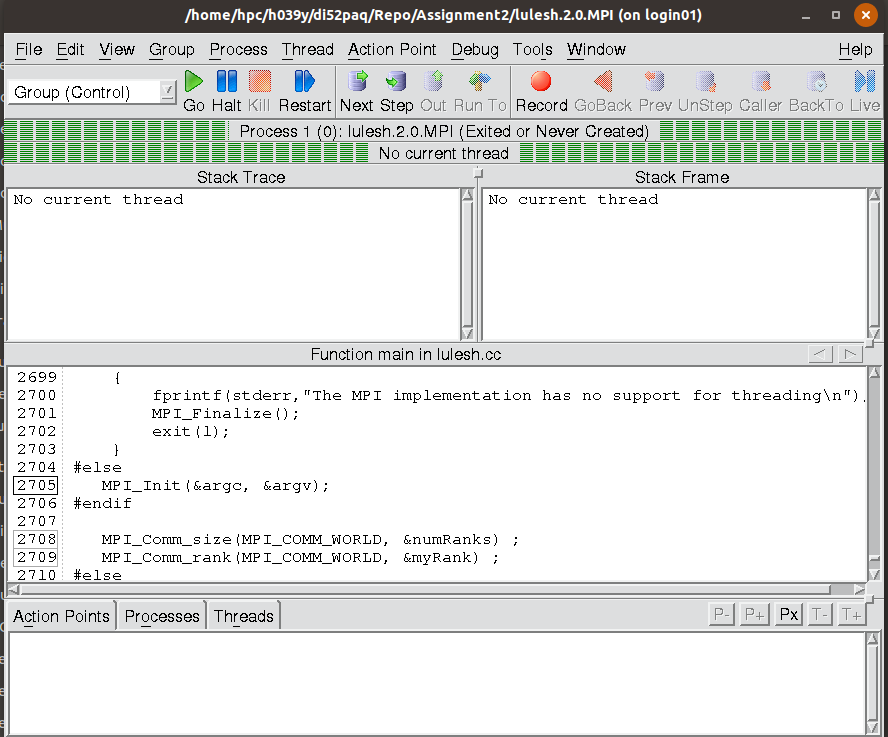
\includegraphics[width=.7\linewidth]{ProcessWindow.png}
		\caption{Process Window}
		\label{fig:proc_window}
	\end{figure}
	\item Variable Window
	Displays information about a program's objects. Allows user to change the element values or to cast these values (changing how the value is displayed). You can define fields which change how objects are viewed, for example: expression field (views result of a particular expression, ie. viewing a particular element in an array with expression 'val[3]' instead of 'val'.); type field (changing the data type of the particular element, and so on. The user can also 'dive' into more complex elements to observe or change members of structures or elements of arrays.
	
\end{itemize}
Lorem ipsum

\end{document}

%eof
